%!TEX root = ../thesis.tex
%Adding the above line, with the name of your base .tex file (in this case "thesis.tex") will allow you to compile the whole thesis even when working inside one of the chapter tex files
\vspace{-5mm}
\singlespacing
\chapter{Coronal Mass Ejection Shocks and Particle Acceleration} 
\label{chap:5}
\doublespacing
\vspace{-10mm}
CMEs often erupt at speeds in excess of the local magnetoacoustic wave speeds in the corona. Traveling in excess of Alfv\'{e}n Mach 1, they often drive shocks which can have a variety of physical manifestations, such as radio bursts, coronal bright fronts (CBFs), white-light enhancements, and the in-situ detection of energetic particles. Despite such a variety of shock phenomena being observed for decades, the unifying physical mechanism between these phenomena remains unknown. This chapter will provide an analysis that uses extreme ultraviolet, radio, and white-light imaging of an eruptive event on 22 September 2011 to determine the properties of a CME-driven shock in the corona. The results show that a plasma shock with an Alfv\'{e}n Mach number of $2.4^{+0.7}_{-0.8}$ was coincident with a coronal bright front and an intense metric radio burst generated by electrons with kinetic energies of 2--46 keV. This work provides new evidence to show that the relationship between CMEs, CBFs, and radio radio bursts can be a coronal shock driven by the CME flank. The chapter is based on publications by Carley et al., {\it Nature Physics}, 2013, and Zucca et al., {\it Astronomy \& Astrophysics}, submitted.

\doublespacing
\section{Introduction}\label{sec:1}
Coronal mass ejections (CMEs) 
%are spectacular eruptions of magnetized plasma from the low solar atmosphere into interplanetary space \citep{byrne2010, roussev2012}. With kinetic energies of $\sim$$10^{25}$\,J \citep{vour2010}, they are the most energetic explosive events in the solar system and 
are often associated with plasma shocks and the acceleration of particles to relativistic speeds \citep{klassen2002, grechnev2011}. However, the underlying mechanism relating CMEs, shocks, and particle acceleration is still a subject of intense debate \citep{vrsnak2008}. By clarifying the inherent characteristics of these phenomena we learn not only about the nature of explosive plasma events but also about how they drive shocks and accelerate particles to high energies. The understanding of such processes are important for fundamental solar physics, plasma physics, and space weather predictions.

%ubiquitous in the universe, playing a role in the acceleration of cosmic rays in supernovae and active galactic nuclei shocks \citep{drury2012}.


CME-associated shocks are often observed over a variety of spectral bands. At radio frequencies, high intensity ($\sim$$10^8$\,Jy) emissions, known as type II and type III bursts, are associated with coronal shocks and accelerated particles in the solar corona \citep{wild1950, mann1996}. Fine structure in these radio bursts can often reveal a \textquoteleft bursty' nature to the shock particle acceleration \citep{mann2005}, which can reveal details of the internal shock structure \citep{zlobec1993, guo2010}.
At extreme ultraviolet (EUV) wavelengths, the shock or pressure pulse response of the corona to an eruption may be imaged as a bright pulse propagating across the entire solar disk at typical velocities of 200--400\,km\,s$^{-1}$ \citep{gallagher2011}. These \textquoteleft coronal bright fronts' (CBFs) are a regular feature of solar eruptive events and often display wave-like properties such as reflection \citep{gopal2009}, refraction \citep{wang2000} and pulse broadening \citep{long2011}. %
Like CMEs, CBFs are often accompanied by type II and type III radio bursts, with EUV and radio images revealing a spatial link between the phenomena that is suggestive of a common origin \citep{maia2004, kozarev2011, vrsna2005}.


It has been proposed that the common origin for these myriad phenomena may be a CME-driven shock \citep{grechnev2011, warmuth2004b}.  In this scenario, the CME eruption drives a pressure pulse, observable in the low corona as a propagating wave-like CBF. Higher in the corona this same pulse forms a shock, accelerating particles and producing type II and III emission. However, much debate surrounds the suggestion that (i) the CBF is a plasma pressure wave driven by a CME, and (ii) the radio bursts, generated by accelerated particles, result from this same wave/shock system. The contention has arisen from attempts to explain non-wave kinematics of CBFs \citep{zhukov2009}. Pseudo-wave theories are employed to describe this behavior, where the erupting CME produces a large-scale restructuring of the coronal magnetic field, which results in a propagating bright pulse (via Joule plasma heating) that is not actually a driven wave \citep{delannee2008}. In this scenario, any relationship with shock observables is indirect. Further confusion is added by the possibility that high energy particles in association with the eruption may be a consequence of magnetic reconnection in the flaring active region, and not the result of a shock \citep{kahler2007}.

Collectively, CMEs, CBFs and radio bursts provide direct measures of both shock kinematics and the characteristics of the accompanying accelerated particles. However, a common theory explaining these phenomena has yet to be verified.
This lack of clarity can be ascribed to an EUV imaging cadence that was unable to match the fast time sampling of radio imaging and spectroscopy. Now, using the high image cadence of the Solar Dynamics Observatory \citep[SDO;][]{presnell2012}, combined with fast time sampling radio images and spectra, we can reveal previously unseen characteristics of the relationship between these phenomena, proving that a CME-driven shock is the feature unifying these observations and that this shock is responsible for bursty electron acceleration. This greatly advances our understanding of the close relationship between solar eruptions, plasma shocks and their resulting EUV, radio and particle acceleration signatures.


%----------------------------------------------------%
%			CBF and radio source		    %
%											    %	

\section{Coronal Bright Front and Radio Source}\label{sec:10}

%------------------ Observations --------------------%
\subsection{Observations}
On 22 September 2011 at 10:29\,UT, an X-ray flare (GOES class X1.4) began in an active region located on the east limb of the Sun (NOAA active region 11302; N13E78). Approximately 11 minutes after the flare start time, a bright wave-like front (CBF) was observed propagating away from the southern edge of the active region in SDO/Atmospheric Imaging Assembly \citep[AIA;][]{lemen2012} 21.1\,nm passband images. The CBF then propagated along the east limb from $\sim$15$^{\circ}\,$\,south to $\sim$50$^{\circ}\,$\,south of the equator (Figure.~\ref{fig:figure_aia_nrh_c2}). During the same period of the CBF propagation, a bright 150.9\,MHz source formed above the CBF, imaged using the Nan\c{c}ay Radioheliograph \citep[NRH;][]{kerdraon1997} (contours Figure.~\ref{fig:figure_aia_nrh_c2}). 
%
%
\begin{sidewaysfigure}
    \centering
	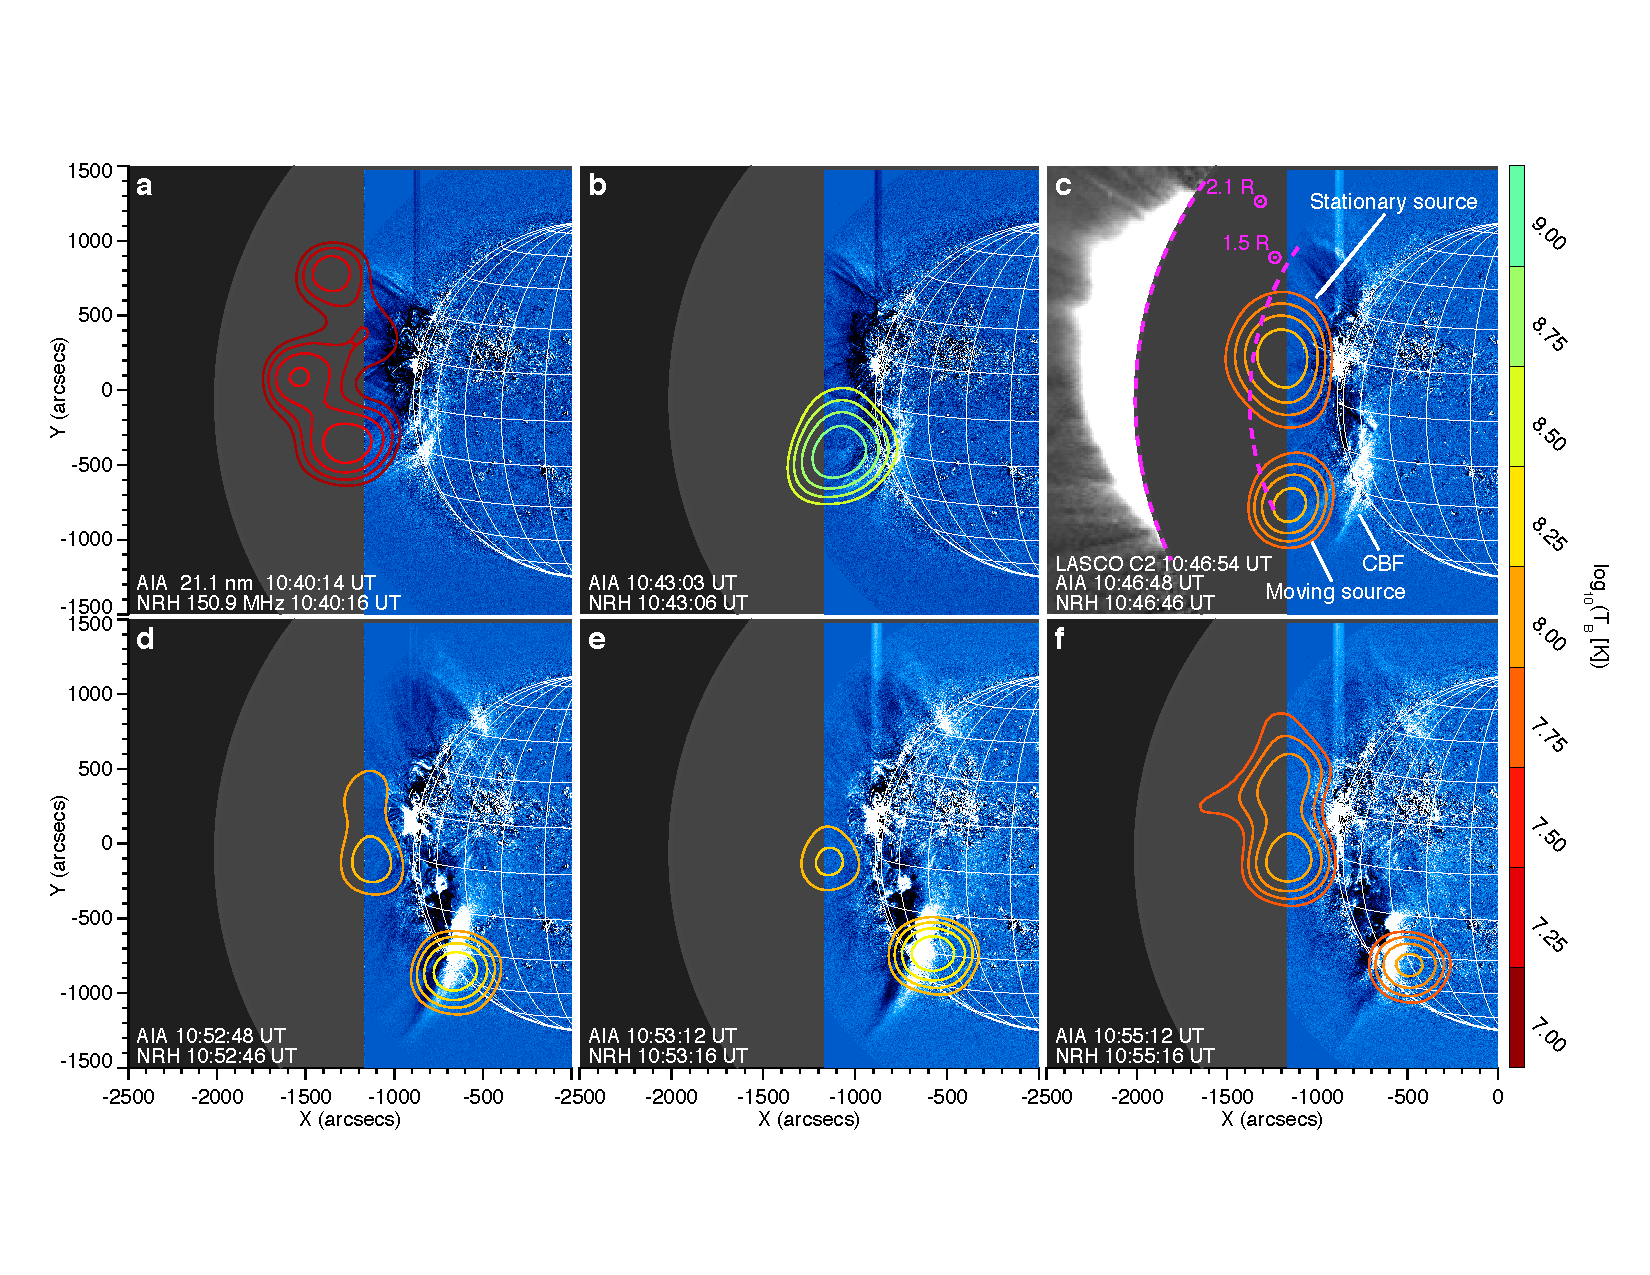
\includegraphics[scale=0.7, trim=0cm 2.5cm 0cm 1.5cm]{gallagher_figure1_final.pdf}
	\caption{{\bf a-f} show that the 150\,MHz source follows closely the coronal bright front (CBF) as it propagates around the east limb, indicating they belong to a common structure. The intensity of the radio source is indicated by the colour bar on the right. {\bf c} reveals the role of the CME in the event, as observed by the LASCO C2 coronagraph. The combination of the white-light coronagraph (C2) and the EUV images (AIA) reveal the full spatial extent of the CME bubble i.e., the frontal structure in white-light has clear extensions back toward the solar surface, imaged at EUV. The location of the radio source and CBF show they clearly have a relationship with the southward CME flank.}
	\label{fig:figure_aia_nrh_c2}
\end{sidewaysfigure}
%
%
In each image the contours range from $T_{peak}$ to $0.95T_{peak}$, where $T_{peak}$ is the peak brightness temperature at the time of the image; the intensity of the contours is indicated by the colour bar on the right. Initially, both the erupting structure seen in the AIA image and the radio source had the same spatial extent over latitude (Figure.~\ref{fig:figure_aia_nrh_c2}a), showing they belong to a common structure. After this, the most southern part of the radio source reached an extremely high brightness temperature ($\sim$10$^9$\,K) and closely followed the propagation of the CBF southward until it eventually diminished into the thermal background at 10:56\,UT. Another emission source at 150.9\,MHz was also observed at $\sim$$0^{\circ}$ latitude on the east limb at a height of 1.1--1.3$\,R_{\odot}$ (Figure.~\ref{fig:figure_aia_nrh_c2}c,d,e,f); while this source was clearly associated with the eruptive active region, any link between it and the CBF is secondary, as it shows no temporal relationship with the start and stop time of the bright front. Similar radio source motion is observed at 173, 228 and 270\,MHz, however any co-propagation of these radio sources with the CBF is of much shorter duration. Figure.~\ref{fig:figure_aia_nrh_c2}c 
reveals the role of the CME in the event, as observed by the LASCO C2 coronagraph. The combination of the white-light coronagraph (C2) and the EUV images (AIA) reveal the full spatial extent of the CME bubble i.e., the frontal structure in white-light has clear extensions back toward the solar surface, imaged at EUV. The location of the radio source and CBF show they clearly have a relationship with the southward CME flank.

%A movie showing the co-propagation of the CBF and 150\,MHz radio source can be found in Supplementary Movie 1. For a movie and discussion of the multi-thermal nature of the CBF see Supplementary Movie 2.


%-------------- Data Analysis -----------------------%
\subsection{Radio Source Height and Speed}
To compare the motion of the CBF and radio source, the position angle (PA) trajectories were analyzed (Figure.~\ref{fig:angle_time}). Here position angle is measured in degrees counter-clockwise from solar north. The solid lines show a fit of $\theta(t) = \theta_0 + \omega t$ to the data, where $\theta_0$ is the starting PA, $\omega$ is the angular velocity, and $t$ is time. The slope of each line gives $\omega$, from which the velocity of the source may be obtained using $v=r\omega$, where $r$ is the distance of the source from Sun center. 
\begin{figure}[!t]
\begin{center}
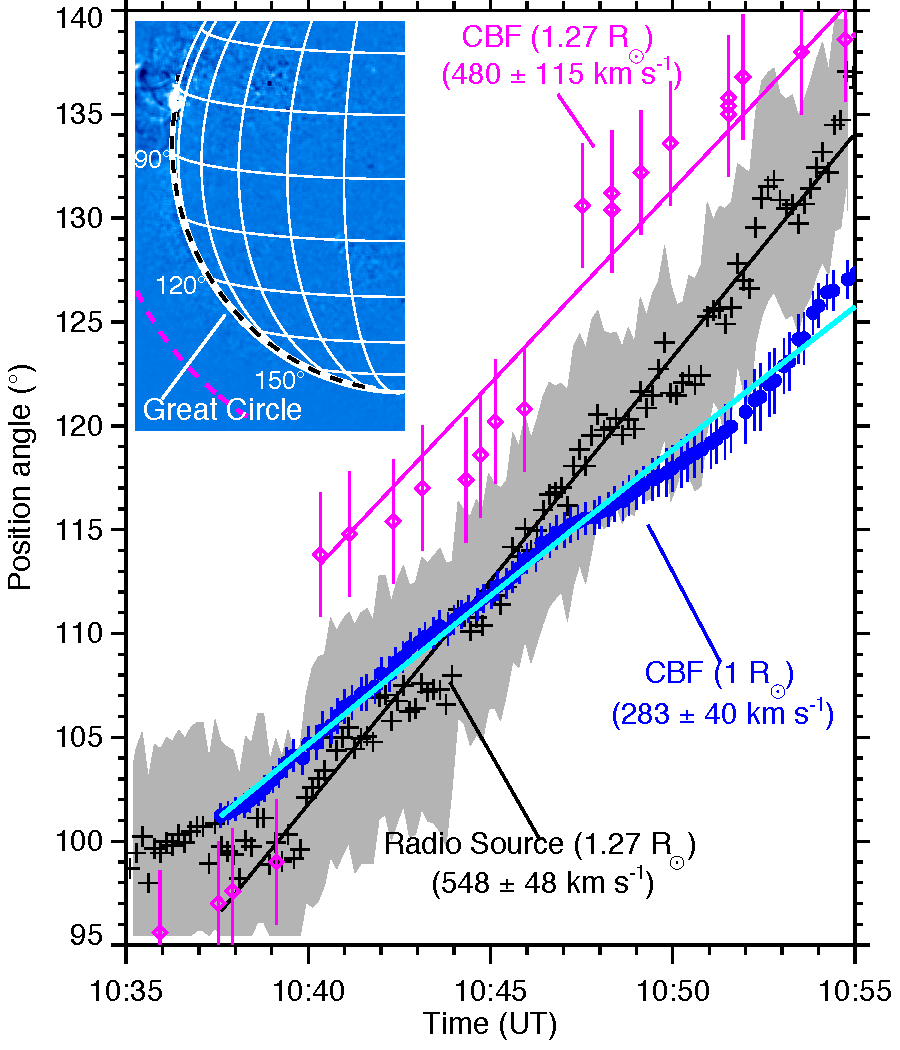
\includegraphics[scale=0.7, trim=1cm 0cm 0cm 0cm]{gallagher_figure2_final.pdf}
\caption[Radio source and CBF position angle versus time]{Position angle (degrees anticlockwise from solar north) versus time for the 150\,MHz source, shown in plus signs, and coronal bright front (CBF) at $1\,R_{\odot}$ (circles) and $1.27\,R_{\odot}$ (diamonds). The great circle along which the CBF was tracked at $1\,R_{\odot}$ is indicated by the dashed white line in the inset; the dashed pink line marks a height of $1.27\,R_{\odot}$. Both radio burst and CBF have a consistent propagation in the same direction and have similar speeds at a height of $1.27\,R_{\odot}$, implying they belong to a common propagating coronal structure. The uncertainty on radio source position angle is taken to be from 1$\sigma$ uncertainties of the source width ($\sim$7$^{\circ}$) plus the fluctuation of source position due to coronal and ionospheric scattering effects ($3^{\circ}$ at frequencies up to 160\,MHz \citep{stewart1982}). The CBF position uncertainty is from Gaussian centroid uncertainty from a tracking and fitting algorithm of the CBF pulse \citep{long2011a}.}
\label{fig:angle_time}
\end{center}
\end{figure}

%----------------- Height of radio source ----------------------%
The 150\,MHz source had an angular velocity of $6.2\pm0.1\times10^{-4}\,\mathrm{rad\,s^{-1}} $. In order to estimate the height of the radio source we first convert from frequency to electron number density using equation~\ref{eqn:plasma_frequency}. Usually, there would be a conversion of this plasma frequency using the density models described in Section~\ref{sec:freq_drift}. However, as outlined, these models can often provide a poor description of the corona and lead to an evaluation of height for the radio burst that may be incorrect. For a more reliable calculation of radio source height we derive density models from data, rather than relying on a `guess' model.

%Given the radio source had a frequency of emission of 150\,MHz, we first convert to density using equation (3) below, and assuming that the emission is harmonic, this results in a density of $n_e=6.9\times10^7$\,cm$^{-3}$. 
Both the LASCO C2 coronagraph and AIA were used for density diagnostics of the corona. Firstly, six AIA passbands were used to create emission measure and density maps of the corona from 1.0--1.3\,$R_{\odot}$ (Zucca et al. 2013), following the method outlined in \citep{asch2013}, details are provided in Appendix~\ref{app:densities}. From 2.0--4.0\,$R_{\odot}$ density diagnostics were performed using the LASCO C2 coronagraph \citep{vdeh50}. Density diagnostics via white-light studies involve the Thomson scattering theory and van de Hulst coefficients, also described in Appendix~\ref{app:densities}. The density diagnostics of AIA and LASCO C2 are combined into a single density image. This results in density values from 1.0--4.0\,$R_{\odot}$, but with a gap in measurement between the two fields of view of the two telescopes (1.3--2.5\,$R_{\odot}$). In order to fill this gap a hybrid of a plane parallel and a spherically symmetric hydrostatic equilibrium (HE) model were fit to the density data from AIA and C2 to form a continuous density map from 1.0--4.0\,$R_{\odot}$. This hybrid model model has the form
\begin{equation}
%n(r) = n_{ar}\mathrm{exp}\bigg(-\frac{\mu m_pgr}{kT}\bigg) + n_{qs}\mathrm{exp}\bigg[\frac{\mu m_pGM_{\odot}}{kTR_{\odot}} \bigg(\frac{R_{\odot}}{r}-1\bigg)\bigg]
n(r) = n_{ar}\mathrm{exp}\bigg(-\frac{r}{H}\bigg) + n_{qs}\mathrm{exp}\bigg[-\frac{1}{H} \bigg(\frac{1}{R_{\odot}}-\frac{1}{r}\bigg)\bigg]
\label{eqn:hybrid_hydro}
\end{equation}
where $r$ is heliocentric distance and $H=kT/\mu m_pg_{\odot}$ is the scale height, where $T$ is temperature, $k$ is Boltzman's constant, $m_p$ is a proton mass, $\mu$ is mean molecular weight, and $g_{\odot}$ is acceleration due to gravity at $1\,R_{\odot}$. Here, the plane parallel model for $n_{ar}$ corresponds to the active region of the data derived from the EUV images, while the spherically symmetric model corresponds to the quiet corona ($n_{qs}$) C2 data. A spherical symmetric model is used for the coronagraph data because the range in heights given by the C2 data will be associated with decreasing gravity (as opposed to the constant gravity over the active region height range). This density model is fit for every position angle such that a 2D map of electron density values in the corona may be obtained (Figure~\ref{fig:density_map}).
\begin{figure}[t!]
\begin{center}
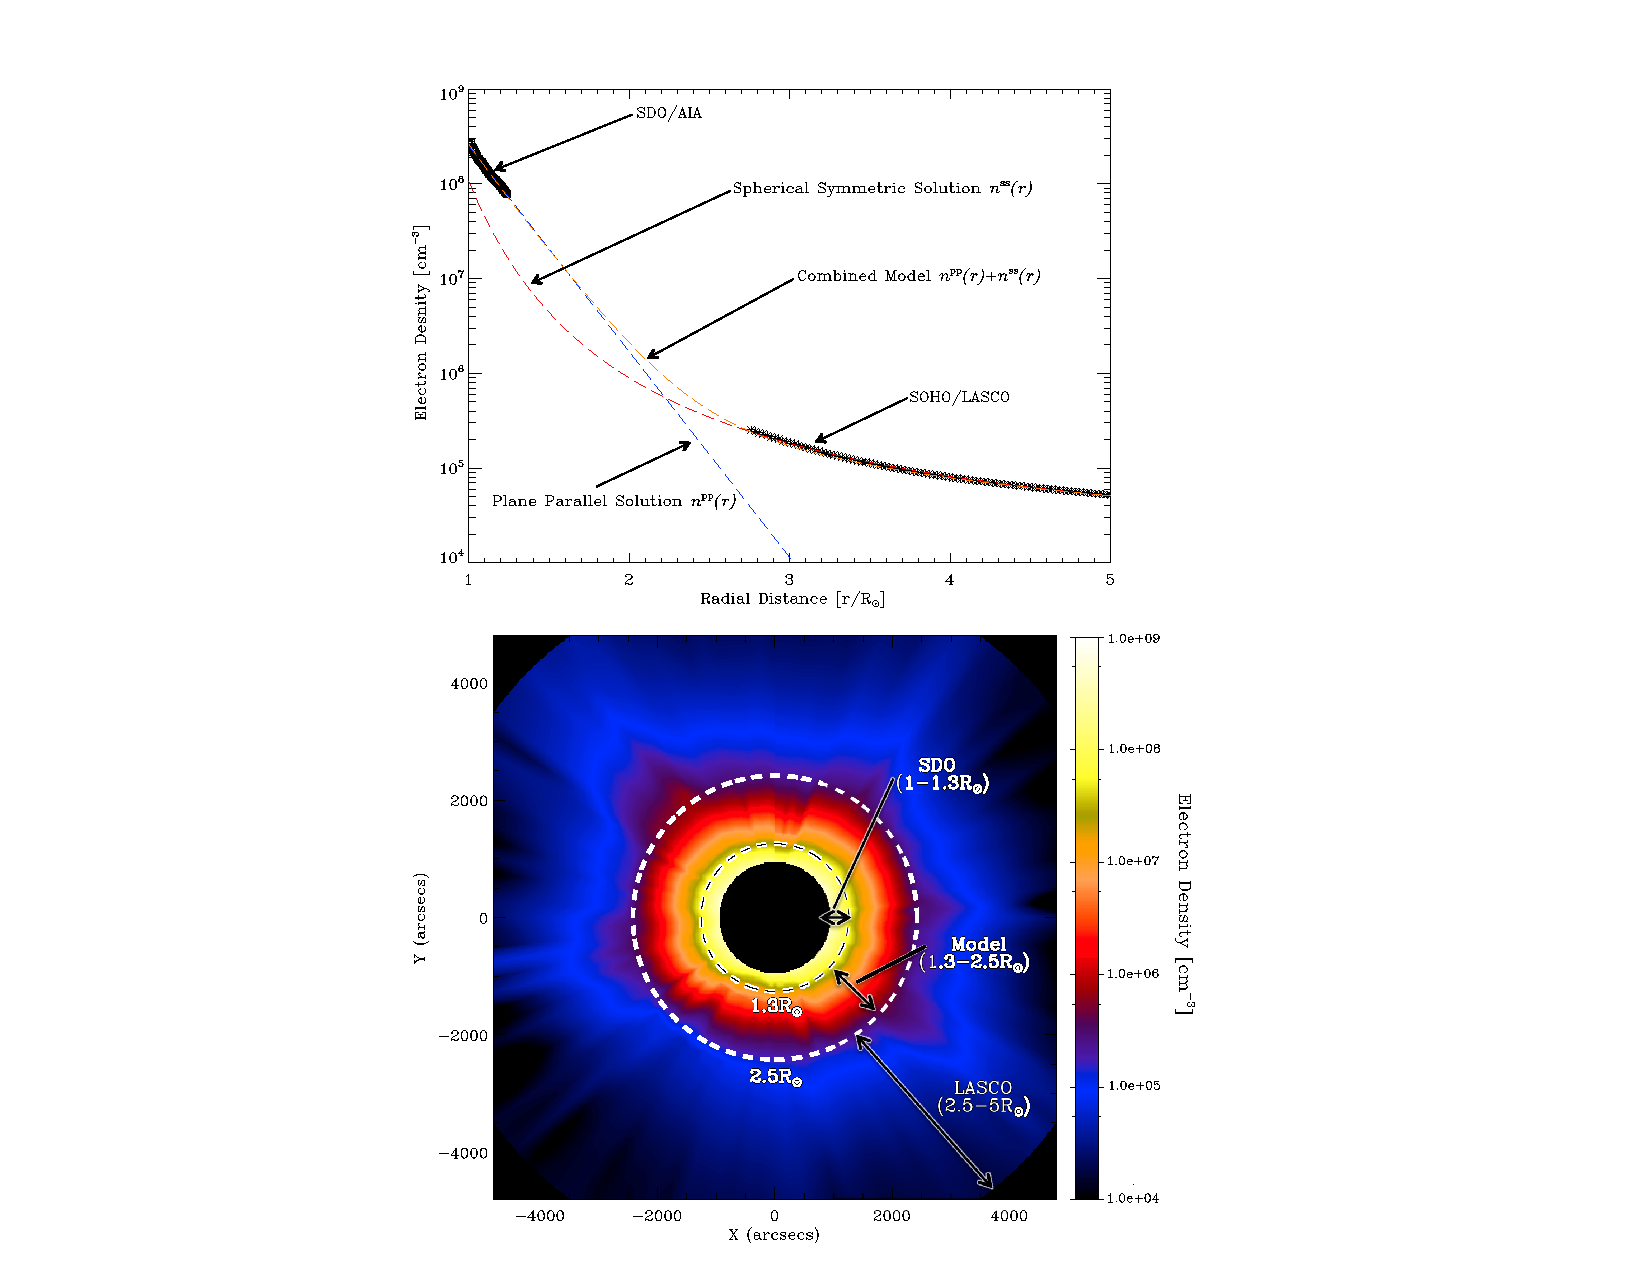
\includegraphics[scale=0.8, trim=4cm 0cm 0cm 1cm]{pietro_density.pdf}
\caption[2D density map of the corona]{(Top) A single radial trace showing the density data derived from AIA and C2. The plane parallel model (blue dash), spherically symmetric model (red dash), and hybrid model (orange dash) are indicated. Mean molecular weight of 0.6 and temperature of $1.4\times10^{6}$\,K were used in Equation~\ref{eqn:hybrid_hydro} (Bottom) A 2D density map created from the hybrid model applied to density data at all position angles 
Density maps such as this can provide much better estimates of radio source height, rather than using a density model which may provide a poor description of the corona.}
\label{fig:density_map}
\end{center}
\end{figure}

These density diagnostics allowed a determination of the height from which 75\,MHz originated (assuming that 150\,MHz observations are of harmonic plasma emission). We find that over the range of the position angles encountered by the radio source (100-140$^{\circ}$), this frequency occurs at an average height of $1.27\,R_{\odot}$, with a maximum height of $1.31\,R_{\odot}$ and a minimum height of $1.21\,R_{\odot}$. We must also take into account that the density measurements themselves have an uncertainty. To account for this, we add the measurement uncertainty (15\%) to the density values and determine the maximum possible height of 75\,MHz in the position angle range, then we subtract 15\% from the density values and measure the minimum possible height. This results in a heliocentric distance of $1.27^{+0.06}_{-0.09}\,R_{\odot}$ for the radio source. This position, including uncertainties, combined with the value for angular velocity ($6.2\pm0.1\times10^{-4}\,\mathrm{rad\,s^{-1}} $) gives the tangential velocity of $548^{+34}_{-48}$\,km\,s$^{-1}$ for the radio source.


\subsection{Radio Source Alfv\'{e}n Mach}

To determine whether or not the radio source motion super-Alfv\'{e}nic, the Alfv\'{e}n speed of the environment through which it propagated was estimated. An estimate of the Alfv\'{e}n speed requires a measure of density (which was derived above) and magnetic field using 
\begin{equation}
v_A = \frac{B}{\sqrt{4\pi n_p \mu m_p}}
\end{equation}
where $B$, $\mu$ is the mean molecular weight taken to be 0.6 for the corona, $n_p$ is the proton number density (same as electron number density for fully ionized hydrogen plasma), and $m_p$ is proton mass. To estimate the magnetic field strength, we used a potential field source surface (PFSS) extrapolation of the coronal magnetic field on the 22-Septemper-2011 06:04\,UT, shown in Figure~\ref{fig:pfss}. 
This was performed using the SolarSoft package of \citet{schrijver2003} and data from the Helioseismic and Magnetic Imager (HMI)\citep{scherrer2012} of the SDO spacecraft. Green and pink lines signify open field regions while white is closed field.
\begin{figure}[t!]
\begin{center}
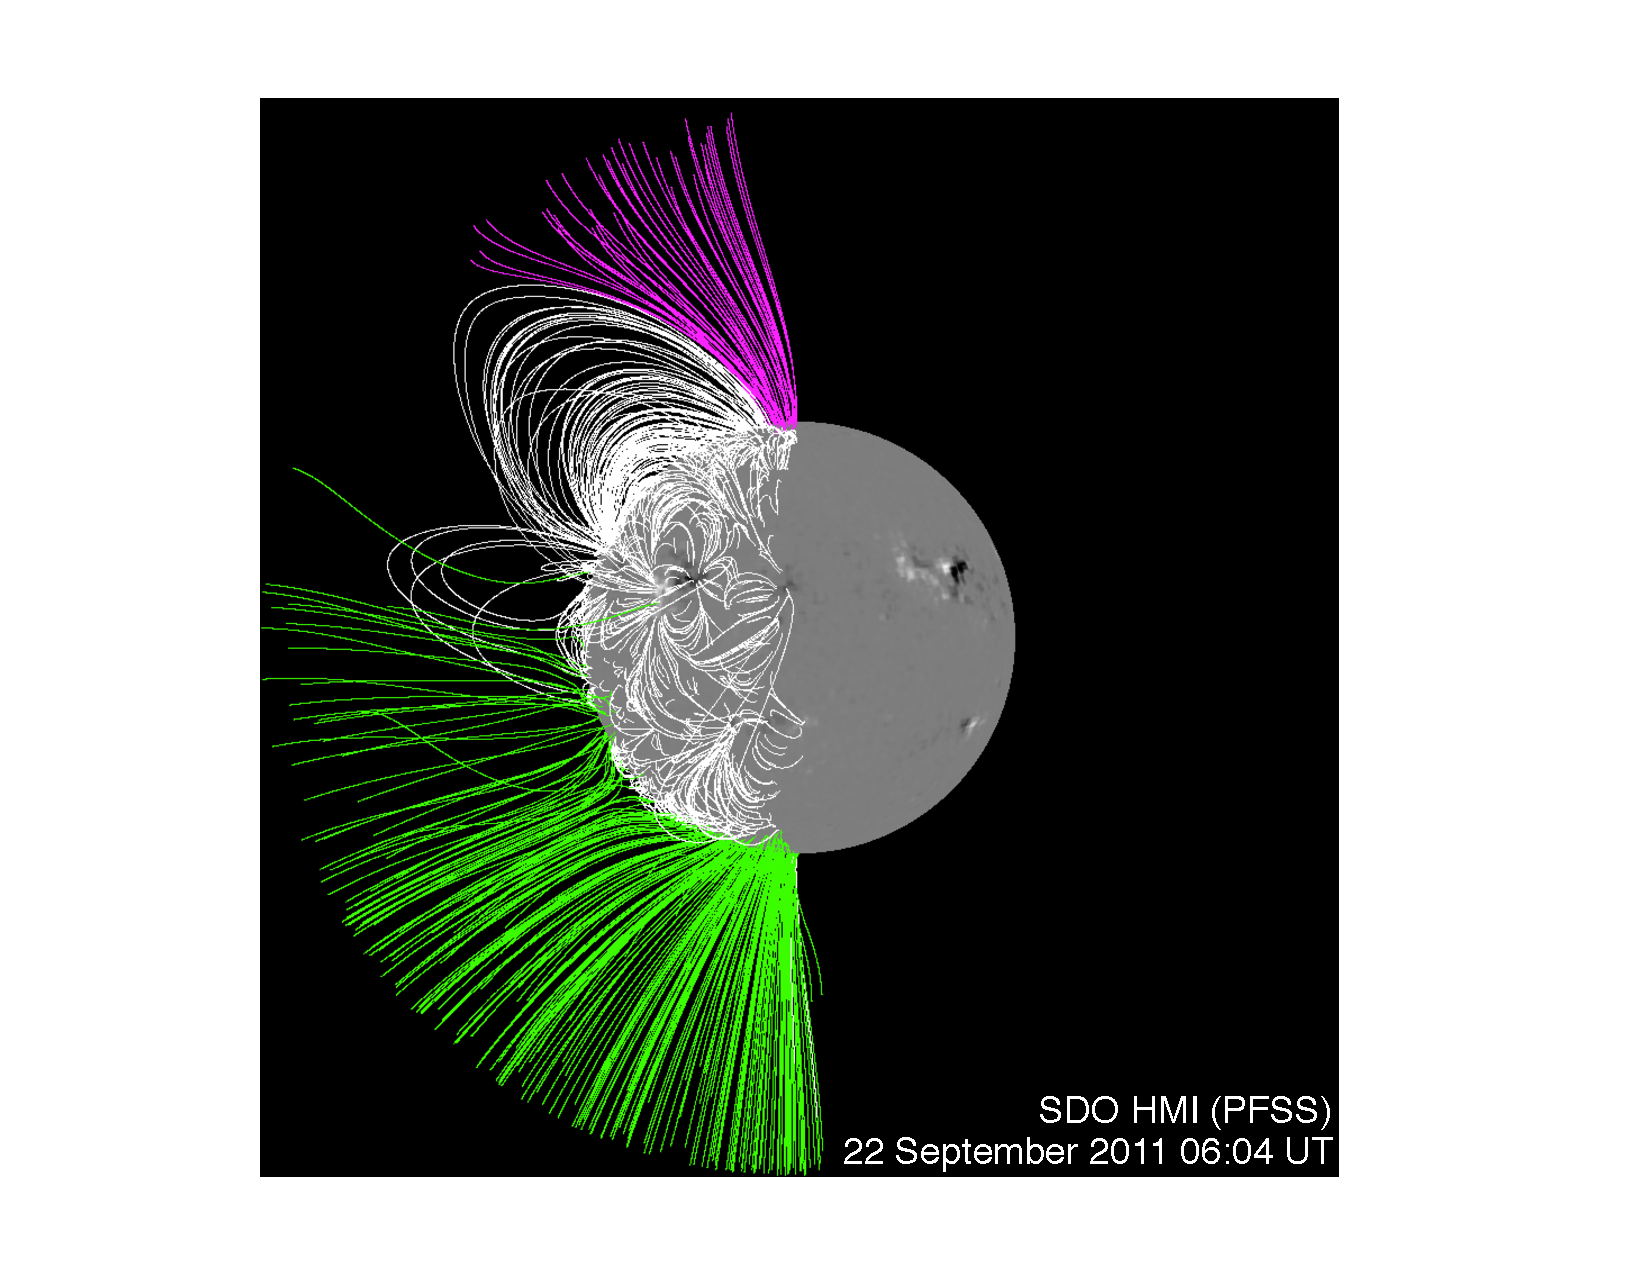
\includegraphics[scale=0.6, trim=1cm 1cm 0cm 1cm]{gallagher_supplem_fig2_final.pdf}
\caption[A potential field source surface extrapolation of the corona magnetic field]{A potential field source surface (PFSS) extrapolation of the coronal magnetic field on the 22-Septemper-2011 06:04\,UT. This was performed using the SolarSoft package of \citet{schrijver2003} and data from the Helioseismic and Magnetic Imager (HMI)\citep{scherrer2012} of the SDO spacecraft. Green and pink lines signify open field regions while white is closed field. The CBF and CME flank propagated through the south-east quadrant. Therefore a transverse propagation through these open and closed field structures suggests that the shock was likely of quasi-perpendicular orientation.}
\label{fig:pfss}
\end{center}
\end{figure}
The PFSS extrapolation provides magnetic field was combined with the density map to produce a 2D Alfv\'{e}n speed map of the corona, such that the Alfv\'{e}n speed position may be obtained for any position in the 2D sky-plane. This is the first time such empirical values of density and magnetic field have been produced for the 2D sky-plane. 
At the source heliocentric distance of $1.27\,R_{\odot}$ we find $B=0.67$\,G. Combining this with the density at the radio source results in an Alfv\'{e}n speed of $225$\,km\,s$^{-1}$. 
%
%
%
\begin{figure}[t!]
\begin{center}
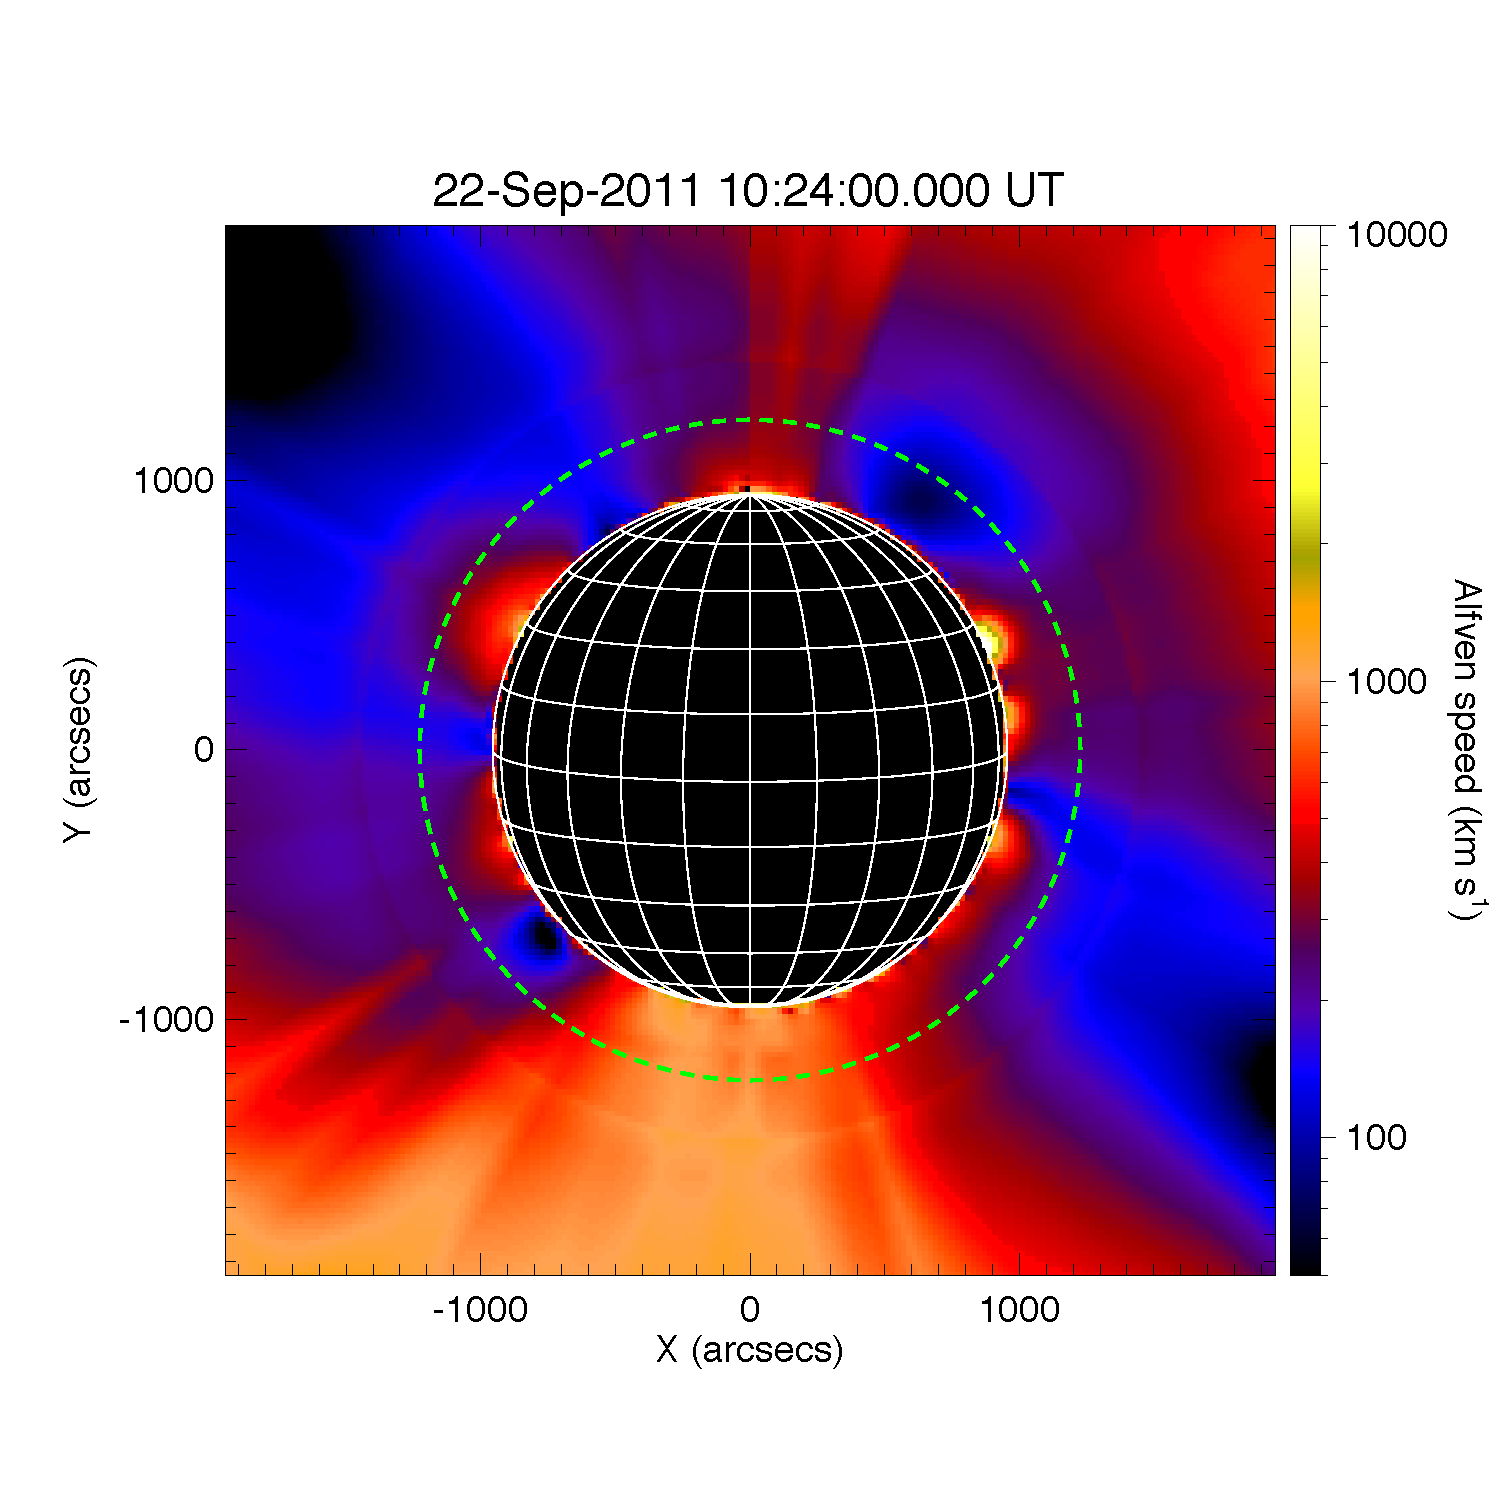
\includegraphics[scale=0.5, trim=1cm 2cm 0cm 3cm]{thesis_alfven_map.pdf}
\caption[Alfv\'{e}n speed map of the solar corona.]{Alfv\'{e}n speed map of the solar corona, derived from density values using LASCO C2, SDO/AIA, and magnetic field values from the PFSS extrapolation. These empirical observations have features which were predicted by the model Alfv\'{e}n produced by \citet{warmuth2005} i.e., the presence of minima in Alfv\'{e}n speed close to active regions. The greed circle marks a height of 1.27\,$R_{\odot}$. Figure adapted from Zucca \& Carley\,{\it et.\,al.} (submitted)}
\label{fig:pfss}
\end{center}
\end{figure}
%
%
%
Taking into account that the source may be in the range from $1.18-1.33\,R_{\odot}$, we find a possible range of $0.5-0.9$\,G for the magnetic field that the source may encounter between the position angles of $100-135^{\circ}$. Again using the density at the radio source we find the possible range in Alfv\'{e}n speeds that the source may encounter is $190-310$\,km\,s$^{-1}$. Hence we quote the Alfv\'{e}n speed as $v_A=225^{+85}_{-35}$\,km\,s$^{-1}$. Using the speed of the source we then find the Alfv\'{e}n Mach to be $M_A =2.4^{+0.7}_{-0.8}$. We note that it is not possible to estimate an error on the magnetic field strength since it is an extrapolation from the surface field, however, the results of super-Alfv\'{e}nic Mach are tolerant to within 50\% uncertainty on the PFSS B-field estimate. Also, the PFSS represents the lowest energy state of the coronal magnetic field, hence this Mach number is taken to be an upper limit.

Finally, the direction of the field is also given by the PFSS extrapolation. It shows an extended region of open and radial field structure in the south east quadrant of the corona, with a weak closed field region on disk in this quadrant. The shock propagated transversely through this region, showing there is a strong possibility of the shock encountering quasi-perpendicular orientation of the magnetic field. As was described in Section~\ref{sec:sda_discussion}, quasi-perpendicular orientation is an essential aspect of the SDA process and generation of plasma emission


\subsection{CBF Speeds}
In a similar approach to the radio source motion, the CBF motion was tracked along a great circle at the solar limb to obtain its position angle trajectories with time Figure~\ref{fig:angle_time}. These positions are shown as blue circles in Figure~\ref{fig:angle_time}. The solid blue line shows a fit of $\theta(t) = \theta_0 + \omega t$ to the data, where $\theta_0$ is the starting PA, $\omega$ is the angular velocity, and $t$ is time. Again, the slope of each line gives $\omega$, from which the velocity of the source may be obtained using $v=r\omega$, where $r$ is the distance of the source from Sun center. 
For the CBF, an angular velocity of $4.1\pm0.4\times10^{-4}$\,rad\,s$^{-1}$ was obtained, resulting in a velocity of $283\pm40$\,km\,s$^{-1}$ at $1\,R_{\odot}$. Although the radio source and CBF show a consistent propagation southwards, the CBF does so at a slower speed, possibly because it is at a smaller height than the radio source. To compare the motion of the CBF and radio source at the same height, the CBF motion was tracked at $1.27\,R_{\odot}$. The CBF was much fainter and more diffuse at this height, hence their are fewer data points and the errors are larger than the $1\,R_{\odot}$ data. At $1.27\,R_{\odot}$, the CBF was found to have an angular velocity of $5.4\pm1.3\times10^{-1}$\,rad\,s$^{-1}$, resulting in $v=480\pm115$\,km\,s$^{-1}$. Both the CBF and radio source clearly show common kinematics at a similar height of $1.27\,R_{\odot}$, with the two features having a consistent progression southward around the east limb. 

\subsection{CBF Thermal Properties}
\begin{figure}[t!]
\begin{center}
\includegraphics[scale=0.52, trim=0cm 10cm 0cm 2cm]{tri_color.pdf}
\caption[Tri-color running ratio images of a CBF.]{Tri-colour running ratio images of the 22-September 2011 CBF, produced from 171, 195 and 211\,\AA~images from SDO. These images are used to discern an general temperature changes of the front as it propagates, with blue color regions indicating a relative cooling, and red/yellow regions indicating a relative heating.}
\label{fig:tri_color}
\end{center}
\end{figure}
In order to investigate any thermal properties of the CBF we have produced tri-colour running ratio images of the CBF, shown in Figure~\ref{fig:tri_color}. A ratio image is one in which the image of interest is divided by a pre-event image e.g., the one direct preceding the image of interest. Any intensity increase will show up as a brightness enhancement. A tri-colour running ratio image is one where three separate filters are used to represent running a running ratio in the the three channels of a Red-Green-Blue (RGB) image. The assignment of the RGB color channels are 171 (blue), 193 (green), and 211� (red). As described in detail in \citet{downs2012}: {\it ``a particular offset in the relative phases or amplitudes of the perturbation for each channel will be spread across the RGB color plane. By nature this representation highlights anticorrelated ratio phases as having strong color components. Correlated phases on the other hand will be confined to a mostly gray-scale range."} 

Since each filter used in the images is sensitive to different temperature ranges a tri-colour movie may indicate a local temperature change due to a passing transient. For example, a positive temperature perturbation (heating) may show up as excess emission in 19.3\,nm and/or 21.1\,nm passbands resulting in a orange/yellow appearance. A negative temperature perturbation (cooling) will result in excess 17.1\,nm channel (6.3$\times$10$^5$\,K) combined with a deficiency in 19.3\,nm (1.2$\times$10$^6$--2$\times$10$^7$\,K) and 21.1\,nm ($\times$10$^6$\,K) channels; this results in a blue appearance in the image. In this way, we can qualitatively identify what parts of the CBF are due to local heating and what parts are due to cooling \citep{cohen2009, downs2012, cheng2012}. The furthermost front has a yellow appearance, indicative of a positive temperature perturbation, with a secondary blue (cooler) front behind it. This is the expected behaviour of a propagating pressure pulse i.e., a traveling pressure perturbation will result in a slight heating followed by a rarefaction and cooling in its wake \citet{downs2012}. This is further confirmation that the CBF observed in this event is indeed a pressure pulse, making it more likely to be associated with shock activity higher in the corona.

\section{Radio Dynamic Spectra}\label{sec:20}

While the NRH imaging data reveal there was a high intensity radio source closely associated with the CBF, the radio dynamic spectroscopy reveal exactly what kind of radio activity this is. Section~\ref{sec:freq_drift} shows that different types of physical activity in the corona, such as particle acceleration and shock activity can be recognised by their characteristic signature in dynamic spectra. 

\subsection{Observations}
The 150\,MHz source observed by NRH had a brightness temperature of $\sim$$10^9$\,K, indicating coherent plasma emission. As decribed in Sections~\ref{sec:wave_particle}--\ref{sec:three_wave}, plasma emission is generated via plasma oscillations that are due to instabilities in the presence of high velocity electron beams. The presence of electron beams was independently verified and revealed in detail using radio dynamic spectra. At $\sim$10:40\,UT the fundamental and harmonic bands of a type II burst shock signature was observed at 45 and 90\,MHz (Figure~\ref{fig:dyn_spec}b), respectively, using the Nan\c{c}ay Decametric Array \citep[NDA;][]{boischot1980}. Type III bursts begin at the same time as the type II (Figure~\ref{fig:dyn_spec}a,b), observed using NASA's STEREO-B/WAVES instrument \citep{bougeret2008}. The speeds of these particles could be obtained from their frequency drift.

\subsection{Particle speeds and in-situ detection}
The frequency drift of these type III radio bursts provide a measure of velocity of the electrons causing the radio emission by converting frequency-time measurements to height-time via a coronal density model. From the dynamic spectra, it is possible to obtain a set of frequency time measurements $(f_i,t_i)$, in this case along the left edge of the type III. Using the expression for plasma oscillation (Equation~\ref{eqn:plasma_frequency}), the set $(f_i,t_i)$ may be converted into a set of density time values $(n_i,t_i)$. In order to convert these into a height-time set $(r_i,t_i)$, a density model of the solar corona is used. The density model in this case is derived from a solution to the Parker solar wind equation which is used specifically to analyze low frequency (interplanetary) type IIIs \citep{Mann1999}. Once this $(r_i,t_i)$ height-time set was found, we took into account that the electron beams are traveling along open magnetic field lines which follow the Parker spiral. In cylindrical coordinates, the radius $r$ and azimuthal angle $\phi$ share the relationship $r-r_0= -\frac{v_{sw}}{\Omega_{\odot}}( \phi - \phi_0)$ i.e., an Archimedean spiral with parameters $v_{sw}$, the solar wind velocity, and $\Omega_{\odot}$, the angular velocity at solar equator. The arch-length along any arm of this spiral (along an open magnetic field line) is given by
\begin{equation}
s(\phi) = \frac{v_{sw}} {2\Omega_{\odot}}\big(\phi\sqrt{1+\phi^2} + \mathrm{arcsinh}(\phi)  \big)
\end{equation}
where arcsinh is the inverse hyperbolic sine function. Using a solar wind velocity value of 450\,km\,s$^{-1}$ (observed in-situ using the STEREO-B PLASTIC)
\begin{sidewaysfigure}[!t]
    \centering
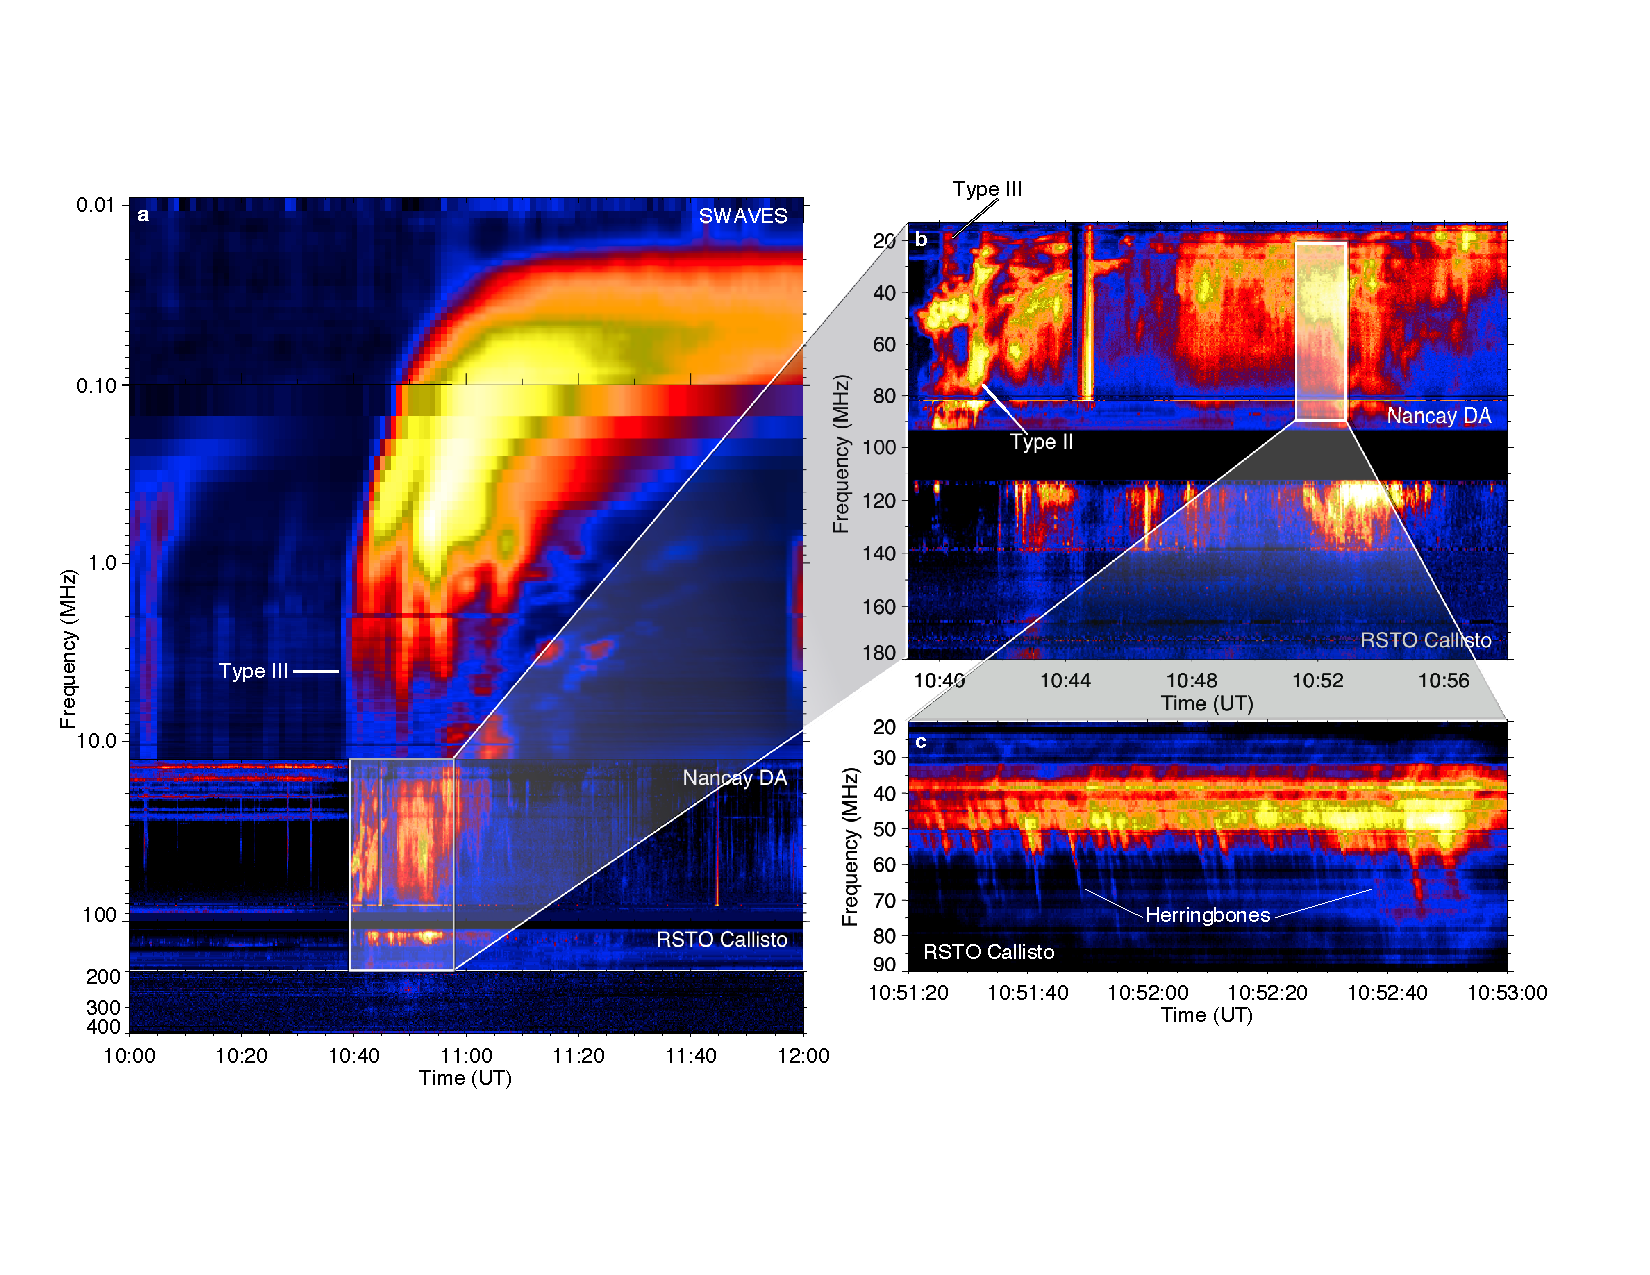
\includegraphics[scale=0.7, trim=0cm 3cm 1cm 4cm]{gallagher_figure3_final.pdf}
\caption{Radio dynamic spectra from STEREO-B/WAVES (0.01--16\,MHz), Nan\c{c}ay DA (20--90\,MHz), and RSTO eCallisto (10--400\,MHz). The type II radio burst is indicated in {\bf b}, with both fundamental and harmonic emission observable. This shock signature is characterized by two emission bands drifting slowly ($\sim$-0.2\,MHz\,s$^{-1}$) toward lower frequency over time. The type III bursts are indicated in {\bf a},{\bf b}, while herringbones are shown in {\bf c}. Each herringbone or is indicative of an electron beam traveling away from the shock. Note that all of the radio activity from {\bf a-c} is indicative of either particle acceleration or a plasma shock in the corona. The start and stop times of this radio activity in these dynamic spectra show good temporal correspondence with the start/stop times of the activity in Figure~\ref{fig:figure_aia_nrh_c2}. This is especially apparent for the features between 100--200\,MHz.}
\label{fig:dyn_spec}
\end{sidewaysfigure}
\clearpage
\noindent
and $\phi=\frac{ \Omega_{\odot}}{v_{sw}}r=-6.5\times10^{-12}$\,rad\,m$^{-1}\times r$, the set $(r_i,t_i)$ were converted to a set of distances along the Parker spiral vs time $(s_i, t_i)$. A linear fit to this data then gives the speed of electrons producing the type III as 0.4\,$c$ (Figure~\ref{fig:typeIII_speeds}). Note that since the $(f_i, t_i)$ points are taken along the left edge of the type III burst, this speed is representative of the fastest electrons contributing to the radio burst. 

It is difficult to estimate an error on this speed, due to a lack of interplanetary density measurements from which this speed is derived, we may confirm the presence of particles with such energy from in-situ data. Figure~\ref{fig:sept} shows a plot of electron flux versus time from the Solar Electron Proton Telescope (SEPT)\citep{muller2008} onboard STEREO-B. It shows an increase in electron flux in the range of 45 - 325\,keV. The vertical black line is the expected time of arrival of the electrons causing the type III burst, calculated from their speed and distance travelled on the Parker spiral. The expected time of arrival of the type III electrons match quite well the first peak in flux of the in-situ detected electrons, showing that the speeds derived from frequency drift are a reliable estimate.

\begin{figure}[!t]
\begin{center}
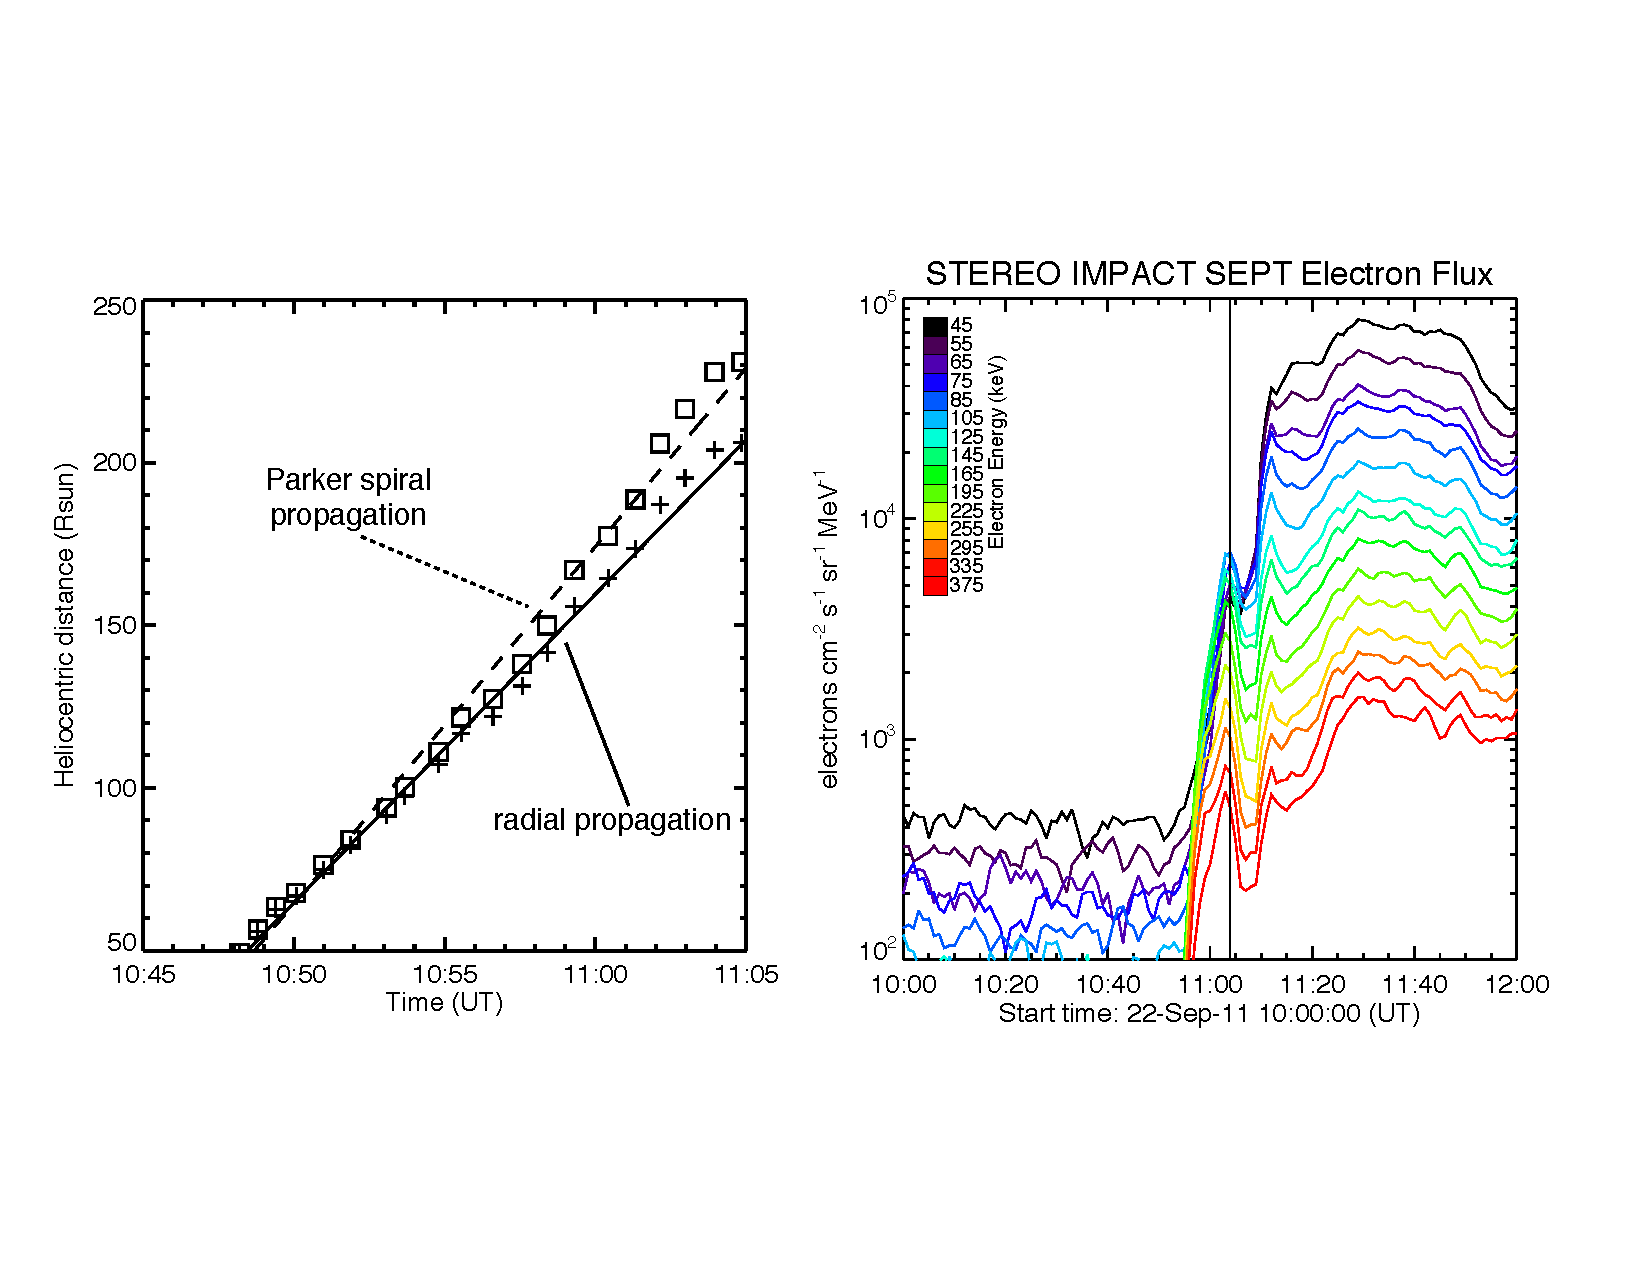
\includegraphics[scale=0.6, trim=1.7cm 4cm 0cm 5cm]{typeIII_speeds.pdf}
\caption[Type III speeds]{(Left) Distance-time for points chosen along the right edge of the type III radio burst observed by S/WAVES. Both radial and Parker-spiral corrected points are shown. (Right) Detection of electrons in-situ by SEPT on STEREO-B. The electrons arrive at $\sim$11:05\,UT, approximately 35 minutes after the flare start time. The black vertical line indicates the expected time of arrival (ETA) of the type III electrons. This ETA was calculated from the electron speed (derived from the frequency drift and a density model), and the distance travelled along the Parker spiral (given a solar wind speed of 450\,km\,s$^{-1}$). Note that the type III electrons, calculated to have an energy of 46\,keV, have an ETA that is centered on the first peak in electron fluxes as detected by the SEPT low energy channels at 45\,keV. This good agreement between predicted ETA and observed time of arrival, showing the type III electron energies are a sound estimate.}
\label{fig:typeIII_speeds}
\end{center}
\end{figure}

More striking evidence for shock-accelerated electrons is in the form of `herringbone' emission, observed using the eCallisto spectrometers \citep{Benz2009} at the Rosse Solar Terrestrial Observatory \citep[RSTO;][]{zucca2012} (Fig.~\ref{fig:dyn_spec}c). The herringbones result from individual beams of shock-accelerated electrons \citep{mann2005}, traveling towards and away from the Sun  i.e., to higher and lower frequencies. Similar features occur between 100--200\,MHz (Fig.~\ref{fig:dyn_spec}b), showing the same characteristics as herringbones (a bursty nature and decreasing intensity with respect to time). In a similar manner to the type III bursts, the beam velocity of herringbone electrons was estimated to be 0.15\,c, again showing the presence of near-relativistic electron acceleration in association with the presence of a shock. 
\begin{figure}[!t]
\begin{center}
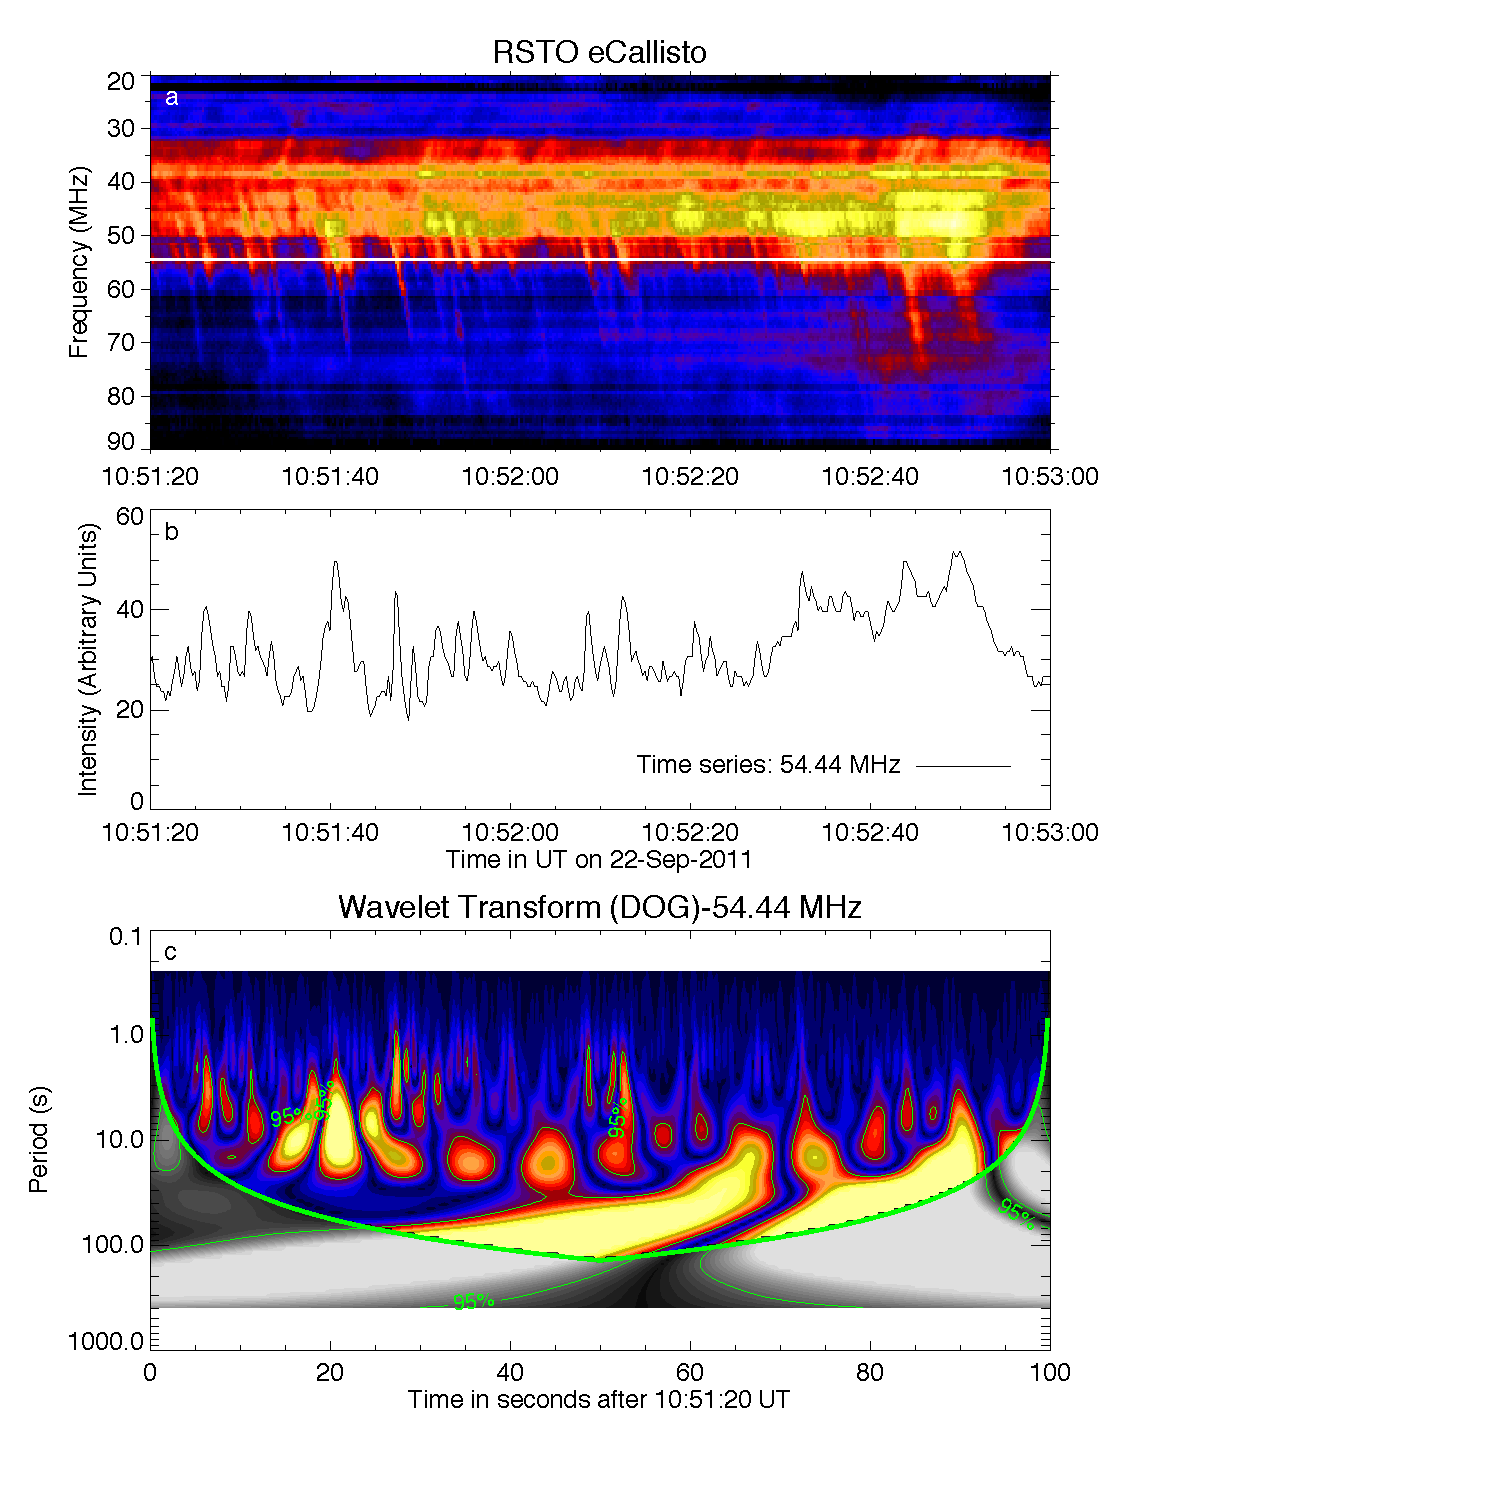
\includegraphics[scale=0.6, trim=0cm 0cm 5cm 1cm]{gallagher_supplem_fig1_final.pdf}
\caption[Herringbone wavelet analysis]{Wavelet analysis of herringbone radio bursts. Panel {\bf a} shows the herringbones, the white line is the frequency from which a time-series has been extracted (54.44\,MHz). Panel {\bf b} shows the time series. Panel {\bf c} shows a wavelet analysis of the time series using a derivative of a Gaussian (DOG) wavelet. The shaded grey area is the region outside the cone of influence and the green contours mark the 95\% confidence level. The wavelet transform shows power in the regions of 2-11 seconds, revealing strong levels of periodicity throughout the time series.}
\label{wavelet}
\end{center}
\end{figure}

While their structure in frequency reveal how fast these beams travel, their behavior in time can reveal detailed temporal characteristics of the shock acceleration process.
A wavelet analysis using a derivative of a Gaussian wavelet performed on a time series at 54\,MHz reveals periodicity at 2--11~seconds (see Supplementary Figure 1). Previous authors have attributed this bursty nature to rippling and inhomogeneity along the shock front, possibly revealing some level of instability or shock turbulence in the acceleration region \citep{burgess2006, guo2010}; we discuss this in the last section. We note that the features at 100--200\,MHz appear to be the extension of the herringbones into higher frequencies. These features in particular show good temporal correspondence with the radio source i.e., they have a start-stop time comparable to the radio source. This is particularly apparent for the group of bursts at 10:52--10:56\,UT.

The radio emission in the dynamic spectra have all the hallmarks of shock generation with particle acceleration closely tied to the process. The association of shock radio activity with the imaged 150\,MHz source suggests that the two observables have a common origin in a plasma shock. Overall, the position of the radio source at the southern flank of the CME, the transverse motion of the source (propagation parallel to the surface) and the zero frequency-drift of the herringbones is suggestive of a shock driven parallel to the surface by the flank expansion, similar to the assertion by \cite{stewart1980} and \cite{schmidt2012}. Indeed the association of the CBF with this radio activity is corroborative evidence of the wave/shock system at the flank. Further evidence of a shock having occurred in the corona was obtained through white-light observations, allowing us to study the position of this shock relative to the CME.

\section{White-light CME and Shock}
\begin{figure}[!t]
\begin{center}
\includegraphics[scale=0.6, trim=2.5cm 1cm 0cm 1.5cm]{gallagher_figure4_final.pdf}
\caption[3D reconstruction of CME and white-light shock]{White-light CME observations and 3D reconstruction of the CME front. {\bf a} Top-down view of the Heliocentric Earth Equatorial (HEEQ) system, showing the separations and locations of STEREO-B and SOHO spacecraft with respect to the Sun. {\bf b} LASCO/C2 base-differenced image of the CME (logged intensity scale), with AIA 21.1\,nm image inset. White crosses indicate a point-and-click along the CME front with a corresponding ellipse fit in blue, where the solid lines indicate the major and minor axes, while dashed lines indicate the apex points back toward the Sun centre. The white circles indicate the white-light shock. The red asterisk points indicate the northern and southern flanks of the CME. {\bf c}, Base difference image of the CME from the COR1-B coronagraph, with a corresponding ellipse fit and EUVI 19.5\,nm image inset. The red lines are the red asterisk points in {\bf b} projected as lines-of-sight across the COR1 field of view. {\bf d} 3D reconstruction of the CME with the white light shock indicated on the plane of sky (only 2D information is available for this feature). The red dotted lines are the projected points from the ellipse on the C2 image, and the blue dotted lines are the projected points from the ellipse on the COR1 image. The black ellipses are those inscribed in the resulting quadrilateral slices via the elliptical tie-pointing method for 3D CME reconstruction, as described in \citep{byrne2010}.}
\label{fig:3d_cme}
\end{center}
\end{figure}
A CME associated with this event was observed by the Large Angle Spectroscopic Coronagraph \citep[LASCO;][]{bru95}, first appearing at 10:46\,UT, with an apex heliocentric distance of $\sim$2.6\,$R_{\odot}$ (Fig.~\ref{fig:figure_aia_nrh_c2}c). The next available image shows the bright CME front with a fainter, secondary front at the southern flank (Fig.~\ref{fig:wl_shock}b). This `two-front' morphology is a common occurrence in white-light CME structure and constitutes a reliable signature of a CME front associated with a stand-off shock \citep{vourlidas2012}. In order to distinguish between the CME front and shock front, we performed a 3D reconstruction of the CME using the elliptical tie-pointing method described in \cite{byrne2010} (Fig.~\ref{fig:wl_shock}d). 

This reconstruction reveals that the bright front outlined in the C2 coronagraph (ellipse in Fig.~\ref{fig:wl_shock}b) corresponds to the faint front outlined as a halo in STEREO-B COR1 (ellipse in Fig.~\ref{fig:wl_shock}c). Furthermore, the observations reveal that the secondary and extremely faint front at the southern edge of the CME (as imaged in LASCO/C2,~Fig.~\ref{fig:wl_shock}b) cannot be considered as part of the CME structure, but is actually an associated shock front. We note that white-light shocks have been reported in the past, occurring both in the low corona as well as out to $\sim$0.5\,A.U. \citep{vourlidas2012, maloney2011}. Here, we have employed a 3D reconstruction from multi-viewpoint observations to qualitatively confirm the presence of a shock at the southern flank of the CME, in the same region as the CBF and radio burst. Finally, a height time analysis of this CME showed that there was no acceleration in the C2 and C3 fields of view, with the CME having a constant velocity of $\sim$1300\,km\,s$^{-1}$.


\section{Discussion}

\subsection{Relationship Between CME, CBF, and Radio bursts}\label{sec:31}

There has been much debate surrounding the assertion that CBFs are a wave phenomenon \citep{gallagher2011}, with numerous authors suggesting a pseudo-wave theory \citep{delannee2008}. In the past, the association of CBFs with type II and type III bursts has been used as evidence against this pseudo-wave interpretation and more in favor of the MHD wave paradigm \citep{warmuth2004b, grechnev2011}. This study reveals that the CBF in this event was indeed closely associated with shock radio activity positioned on the flanks of an expanding CME. This kind of behavior has been suggested before, but never directly imaged \citep{kozarev2011, feng2012, feng2013}. It shows how a combination of radio and EUV imaging can reveal the evolution of plasmoid driven shocks in the solar atmosphere \citep{bain2012}.

The scenario shown to be the case here, is that the expansion of the CME flanks drove a plasma pressure front through the corona. The low coronal manifestation of this pressure front was a CBF. Higher in the corona this same pressure front steepened into a shock; this shock was responsible for the acceleration of particles. These particles produced radio emission which was observed as a propagating radio source and in dynamic spectra in the form of herringbones. Such a scenario is agreement with a variety of studies that have suggested such a physical mechanism e.g., the schematic of \citep{grechnev2011a} shown in Figure~\ref{fig:shock_cbf}, Figure 7 of \citet{warmuth2004b}, and Figure 3 of \citep{stewart1980}. Our own schematic shows a similar scenario in Figure~\ref{fig:shock_schematic}.

\subsection{Bursty Particle Acceleration}\label{sec:sda_discussion}

Of further interest in this study is the likelihood of a quasi-perpendicular orientation of the shock, as revealed by the PFSS extrapolation. A schematic of the CME, CBF and shock orientation with respect to the coronal magnetic field and particle acceleration is shown in Figure~\ref{fig:shock_schematic}
\begin{figure}
\begin{center}
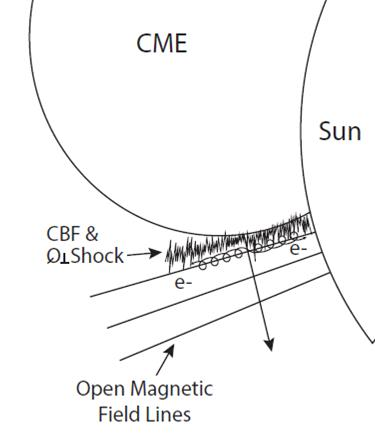
\includegraphics[scale=0.7]{gallagher_schematic.png}
\caption[CBF and shock orientation]{Relationship between the CME, CBF, shock and particle acceleration on the open magnetic field of the ambient corona.}
\label{fig:shock_schematic}
\end{center}
\end{figure}
Quasi-perpendicularity is an essential aspect of the shock drift acceleration (SDA) mechanism \citep{ball2001}, a process believed to be responsible for particle acceleration in planetary magnetospheres \citep{wu1984} and solar radio bursts \citep{holman1983}.
This mechanism involves an adiabatic reflection of particles from the shock, with the energy gain sourced in the $\mathbf{V} \times \mathbf{B}$ electric field, where $\mathbf{V}$ and $\mathbf{B}$ are the upstream flow speed and magnetic field, respectively. A single reflection from the shock has limited energy gain, however multiple reflections may produce relativistic energies, which is particularly important for low Mach number shocks such as that reported here ($M_A =2.4^{+0.7}_{-0.8}$) and in \citep{guo2012}. This multiple reflection process may be explained by inhomogeneity in the shock front, a characteristic usually known as \textquoteleft rippling' \citep{zlobec1993, vandas2011}. 2D hybrid simulations show that rippling is brought about by an instability \citep{burgess2006} and resembles a standing-wave mode of the shock surface \citep{lowe2003}. The presence of ripples can lead to a quasi-sinusoidal variation in shock-normal orientation with respect to the upstream magnetic field. Since the efficiency of SDA requires quasi-perpendicularity, there will be sites on the shock front that provide efficient acceleration and sites that do not $-$ a structure that may lead to magnetic trapping and multiple reflections \citep{zlobec1993}, hence producing higher energy particle acceleration. 

The presence of ripples can produce quasi-periodic herringbones in three ways. Firstly, it makes SDA more efficient and capable of producing the observed herringbone energies, especially when particle scattering is considered \citep{burgess2006}. Secondly, the periodic spatial variation in the acceleration efficiency of the shock could explain the bursty and quasi-periodic nature of the herringbones. \cite{guo2010} suggest that shock front inhomogeneity brought about by MHD turbulence is a possible explanation of bursty herringbones. \cite{schmidt2012} produced a detailed model of SDA from a rippled shock, specifically on the flanks of an expanding CME. Their results suggest that herringbones could be produced by accelerated electrons at spatially intermittent regions of quasi-perpendicularity on a rippled shock surface (Figure~\ref{fig:herbone_model}). Thirdly, \citep{burgess2006} also predicts that, if rippling is present, the upstream and downstream electron beams should have similar energies, which is not predicted for a uniform or \textquoteleft smooth' shock. A sample of the oppositely drifting herringbones in Fig.~\ref{fig:dyn_spec}c shows that positive and negative frequency drifts are both $\sim$5\,MHz\,s$^{-1}$, revealing that the upstream and downstream populations have similar energies (although we note the possibility that both positive and negative drifting herringbone features may be accelerated upstream, as suggested by the schematic of \citep{zlobec1993}). There is also the possibility that the herringbones may be associated with a termination shock of a reconnection outflow occurring behind the CME \citep{aurass2004}. In such a scenario, this shock would have a more indirect relationship with the CME propagation. However, the imaged radio source shows a good temporal correspondence with the shock activity in the dynamic spectra, especially between 10:52$-$10:56\,UT, suggesting the particle acceleration indicated in the spectra shares a close relationship with the propagating source.

Our observations reveal the need for a more detailed modeling of herringbone solar radio bursts. The quasi-periodic behavior of herringbones provides a possible direct measure of shock inhomogeneity and the spatial scales over which the magnetic field varies in the shock and ambient corona; it may also provide a measure of the turbulence in these plasma flows \citep{guo2010}. In the future, high cadence EUV imaging from SDO, combined with sensitive radio imaging-spectroscopy observations from instruments such as the Low Frequency Array \citep[LOFAR;][]{vanHaarlem2013}, will reveal unprecedented detail of plasma shocks and their role in particle acceleration. This may reveal the fundamental nature of a plasma shock process that is universal, but currently impossible to directly observe in any other area of astrophysics. 


